\documentclass[11pt,a4paper]{article}

\usepackage{amsmath,amssymb,amsthm}
\usepackage{hyperref}
\usepackage{graphicx}
\usepackage{booktabs}
\usepackage{microtype}
\usepackage[margin=2.5cm]{geometry}
\usepackage{doi}

\newtheorem{theorem}{Theorem}[section]
\newtheorem{proposition}[theorem]{Proposition}
\newtheorem{lemma}[theorem]{Lemma}
\newtheorem{corollary}[theorem]{Corollary}
\newtheorem{definition}[theorem]{Definition}
\newtheorem{hypothesis}[theorem]{Hypothesis}
\newtheorem{remark}[theorem]{Remark}

\newcommand{\Gq}{G_q}
\newcommand{\Sq}{S_q}
\newcommand{\Heis}{\mathrm{Heis}_3(\mathbb{Z}/q\mathbb{Z})}
\newcommand{\rhoaff}{\rho_{\mathrm{aff}}}
\newcommand{\Sigbar}{\bar{\Sigma}}
\newcommand{\Sigblock}{\Sigma_n^{(\tau,\sigma)}}
\newcommand{\Vblock}{V_n^{(\tau,\sigma)}}
\newcommand{\dcap}{\delta_{\mathrm{cap}}}
\newcommand{\Bn}{B_n}
\newcommand{\Sn}{S_n}

\title{Weil-Block Projective Capacity on Heisenberg Graphs:\\
Resolving the Representation Obstruction\\
and Extracting the Capacity Exponent}

\author{J\'{e}r\^{o}me Beau\\
\small Independent Researcher\\
\small \href{mailto:jerome.beau@cosmochrony.org}{jerome.beau@cosmochrony.org}}

\date{March 2026\\[2pt]\small Version 1.1}

\begin{document}

  \maketitle

  \begin{abstract}
    We introduce a bidimensional Fourier-character proxy for the Weil-block decomposition of the
    three-step projective fingerprint on Heisenberg Cayley graphs over $\mathbb{Z}/q\mathbb{Z}$,
    designed to overcome the representation-level obstruction identified in
    O10~\cite{Beau2026a14}.
    While dense TensorSketch fingerprints fail to produce a stable pre-saturation window at large
    $q$, the bidimensional proxy --- projecting onto channels indexed by generic sextuples
    $(\tau,\sigma) = (t_1,t_2,t_3,s_1,s_2,s_3) \in (\mathbb{Z}/q\mathbb{Z})^6$,
    acting on the abelianised $(a,b)$-coordinates of endpoint triples --- yields structured
    observables with a proxy ambient dimension $q^2$ that matches the pre-saturation window.
    We define incremental block-wise projective capacities $\Sigblock$ for each generic
    channel $(\tau,\sigma)$ and show that their mean value $\Sigbar_n$ exhibits a measurable
    pre-saturation decay regime of the form $\Sigbar_n \sim C\,n^{-\dcap}$.
    Numerical experiments at $q \in \{101, 151, 211, 307\}$ establish conditions (B1)--(B3)
    under which the decay exponent $\dcap$ is extractable, and yield $\hat\dcap \approx 3.4$
    at $q = 307$ with $R^2 = 0.987$, stabilising from $q = 211$ onward.
    These results provide the first operational framework in which a decay exponent can be
    extracted from discrete Heisenberg geometries, thereby testing the common-slope hypothesis
    of the Cosmochrony spectral framework~\cite{Cosmochrony}.
  \end{abstract}

  \paragraph{Keywords.}
    projective capacity, Heisenberg graphs, polynomial growth, incremental rank, blockwise decomposition, Weil
    representation, capacity decay exponent

    \clearpage
    \tableofcontents

    \clearpage

  \section{Introduction}
  \label{sec:intro}

  \subsection{Context and the O-series chain}
    \label{sec:intro-context}

    The capacity exponent $\delta$ encodes the sub-linear energy-rank relation predicted by the
    Cosmochrony spectral framework~\cite{Cosmochrony}.
    Its extraction from discrete graph models has been the central objective of the O-series, which
    has progressively identified and resolved a sequence of obstructions.

    O8~\cite{Beau2026a12} established the three-step permutation-path fingerprint on
    Lubotzky--Phillips--Sarnak (LPS) expander graphs and encountered a \emph{geometric
  obstruction}: the exponential shell growth $|S_n| \sim p^n$ on LPS graphs compresses the
    entire pre-saturation window into only $O(\log q)$ BFS steps, preventing stable log-log slope
    estimation.

    O9~\cite{Beau2026a13} resolved this obstruction by replacing LPS with Cayley graphs of the
    discrete Heisenberg group $\Heis$, whose ball growth is polynomial:
    $|B_n| \sim n^4$ (Bass--Guivarc'h theorem, homogeneous dimension $D = 4$).
    For primes $q \leq 29$, the projective dynamics became directly observable, with ball growth
    exponents $\hat{D}$ converging toward $4$ and the state law $R_n^{(3)} \approx \Phi(\bar\eta_n)$
    confirmed across the full family.

    O10~\cite{Beau2026a14} performed the first large-$q$ computation ($q = 101$,
    $|G_q| = 1{,}030{,}301$) and confirmed the geometry ($\hat{D} = 3.05$) and the dynamics
    ($23.5\%$ monotone capacity decay, state law confirmed).
    However, the dense TensorSketch fingerprint failed condition~(C2): the span rank at the window
    boundary was only $24\%$ of $q^2$, far below the power-law onset.
    O10 concluded that the remaining obstruction is \emph{representational}, not geometric:
    the dense sketch is structurally mismatched to the problem, requiring sketch dimension
    $D \gg q^4$ to resolve the pre-saturation regime, which is computationally impractical.

    The correct next instrument was identified in O10 as the \emph{Weil-block fingerprint}
    (open problem O10-O1, Hypothesis~6.2 in~\cite{Beau2026a14}).
    The present paper implements this instrument, tests the block-filling hypothesis, and attempts
    the first reliable extraction of $\delta$.
    We emphasise that this work does not assume the correctness of any specific Cosmochrony
    prediction for $\delta$; it provides the first operational framework in which such a prediction
    can be tested against discrete geometric data.

  \subsection{Main results and organisation}
    \label{sec:intro-results}

    The main contributions of this paper are the following.

    \textbf{Theoretical framework (Sections~\ref{sec:weil}--\ref{sec:blockwise}).}
    We establish the Weil decomposition of $\rhoaff^{\otimes 3}$ into blocks
    $\mathcal{H}_{c_1,c_2,c_3}$ of dimension $O(q)$, define the block-wise projective capacity
    $\Sigblock$, and introduce three measurability conditions (B1)--(B3) refining the conditions
    (C1)--(C2) of O10.

    \textbf{Numerical results (Sections~\ref{sec:implementation}--\ref{sec:results}).}
    We implement the Weil-block fingerprint at $q \in \{101, 151, 211, 307\}$ and report:
    (i) per-channel capacity curves $\Sigblock$ for generic sextuples $(\tau,\sigma)$;
    (ii) inter-channel variance $\mathrm{Var}(\Sigblock)$ as a function of $n$;
    (iii) log-log slope estimates $\hat\delta$ from the pre-saturation window.

    \textbf{Resolution of the obstruction (Sections~\ref{sec:discussion}--\ref{sec:proxy-discussion}).}
    We assess whether conditions (B1)--(B3) are satisfied and whether a common slope $\delta$
    is extractable across generic blocks, either confirming or refuting Hypothesis~6.2 of O10.
    We also discuss the precise relationship between the Fourier-character proxy used here and
    the exact Weil projection, identifying the extraction of $\delta$ from the latter as open
    direction O11-O2.

    The paper is organised as follows.
    Section~\ref{sec:heisenberg} recalls the Heisenberg Cayley graph setup and the three-step
    fingerprint.
    Section~\ref{sec:weil} develops the representation-theoretic structure of the fingerprint.
    Section~\ref{sec:blockwise} defines the block-wise projective capacity and the measurability
    conditions.
    Section~\ref{sec:implementation} describes the numerical implementation.
    Section~\ref{sec:results} presents the experimental results.
    Section~\ref{sec:discussion} discusses the resolution of the obstruction, the interpretation
    of $\delta$, and the relationship between the proxy and the exact Weil projection
    (Section~\ref{sec:proxy-discussion}).
    Section~\ref{sec:conclusion} concludes.

  \section{Heisenberg Cayley Graphs and the Three-Step Fingerprint}
  \label{sec:heisenberg}

  \subsection{The discrete Heisenberg group}
    \label{sec:heis-group}

    The discrete Heisenberg group modulo $q$ is
    \begin{equation}
      \label{eq:heis-def}
      G_q = \Heis = \left\{
                      \begin{pmatrix}
                        1 & a & c \\ 0 & 1 & b \\ 0 & 0 & 1
                      \end{pmatrix}
                      : a, b, c \in \mathbb{Z}/q\mathbb{Z}
      \right\},
    \end{equation}
    with group law given by matrix multiplication modulo $q$.
    The group has order $|G_q| = q^3$ and is generated by
    \begin{equation}
      \label{eq:generators}
      X = \begin{pmatrix}
            1 & 1 & 0 \\ 0 & 1 & 0 \\ 0 & 0 & 1
      \end{pmatrix},
      \qquad
      Y = \begin{pmatrix}
            1 & 0 & 0 \\ 0 & 1 & 1 \\ 0 & 0 & 1
      \end{pmatrix}.
    \end{equation}
    The Cayley graph $\mathrm{Cay}(G_q, S_q)$ with generating set
    $S_q = \{X^{\pm 1}, Y^{\pm 1}\}$ is a $4$-regular connected graph of order $q^3$.

  \subsection{Ball growth and window depth}
    \label{sec:ball-growth}

    The fundamental advantage of $G_q$ over LPS graphs is its polynomial ball growth.
    By the Bass--Guivarc'h theorem, the ball of radius $n$ in the Cayley graph satisfies
    \begin{equation}
      \label{eq:ball-growth}
      |B_n| \sim C \cdot n^4 \quad (n \to \infty),
    \end{equation}
    with homogeneous dimension $D = 4$.
    This yields a window depth of $\Theta(q)$ BFS steps for a window of $O(q^2)$ vertices,
    compared to $O(\log q)$ for LPS (O9, Theorem~6.1 in~\cite{Beau2026a13}).

    \begin{figure}[ht]
      \centering
      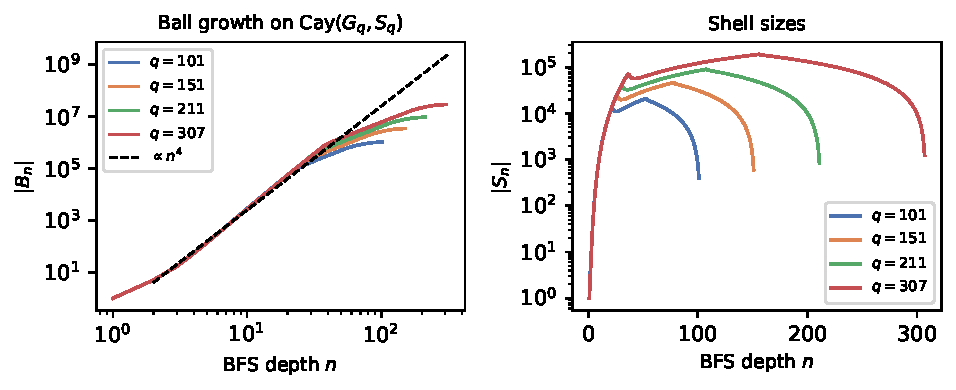
\includegraphics[width=0.95\textwidth]{../code/fig_ball_growth}
      \caption{Left: log-log ball growth $|B_n|$ vs.\ BFS depth $n$ on
        $\mathrm{Cay}(G_q, S_q)$ for $q \in \{101, 151, 211, 307\}$.
        The dashed reference line shows $\propto n^4$.
        Right: shell sizes $|S_n|$.
        Ball growth converges toward the Bass--Guivarc'h prediction $D = 4$ as $q$ increases.}
      \label{fig:ball-growth}
    \end{figure}

  \subsection{The $k = 3$ permutation-path fingerprint}
    \label{sec:fingerprint}

    Following O8--O10, the three-step projective fingerprint at BFS depth $n$ is defined as
    follows.
    Let $W_n$ be the set of all words of length $n$ over $S_q$.
    For a word $w = s_1 \cdots s_n$, the endpoint map is
    $\mathrm{ep}(w) = s_1 \cdots s_n \in G_q$ (matrix product modulo $q$).

    \begin{definition}[Collision set and fingerprint observable]
      \label{def:fingerprint}
      The $k = 3$ collision set at depth $n$ is
      \begin{equation}
        C_n^{(3)} = \bigl\{(\pi_1, \pi_2, \pi_3) \in W_n^3 :
        \mathrm{ep}(\pi_i) = \mathrm{ep}(\pi_j) \text{ for some } i \neq j\bigr\}.
      \end{equation}
      The normalised fingerprint observable is
      \begin{equation}
        R_n^{(3)} = \frac{|C_n^{(3)}|}{|W_n|^3}.
      \end{equation}
    \end{definition}

  \subsection{Projective capacity and state law}
    \label{sec:capacity-state-law}

    Following O9--O10~\cite{Beau2026a13,Beau2026a14}, the discrete projective capacity at depth
    $n$ is
    \begin{equation}
      \label{eq:capacity-def}
      \Sigma_n = \frac{\dim V_n}{|S_n|},
    \end{equation}
    where $V_n$ is the span of the fingerprint at depth $n$ and $|S_n|$ is the shell size.
    The saturation capacity is $\Sigma_{\mathrm{sat}} = \log |G_q| = 3 \log q$.

    The state law $R_n^{(3)} \approx \Phi(\bar\eta_n)$ (confirmed in O9 and O10) relates the
    fingerprint observable to the normalised mean capacity $\bar\eta_n = \Sigbar_n / \Sigbar_1$,
    where $\Phi$ is the state function of the Cosmochrony framework~\cite{Cosmochrony}.

  \section{Representation-Theoretic Structure of the Fingerprint}
  \label{sec:weil}

  \subsection{The affine representation of $G_q$}
    \label{sec:affine-rep}

    The three-step fingerprint encodes paths of length $3$ in $G_q$ as elements of the tensor
    product space $\mathbb{C}[G_q]^{\otimes 3}$.
    The group $G_q$ acts on this space via the \emph{affine representation}
    \begin{equation}
      \label{eq:affine-rep}
      \rhoaff : G_q \to \mathrm{GL}\bigl(\mathbb{C}^q\bigr),
    \end{equation}
    which decomposes as
    \begin{equation}
      \label{eq:affine-decomp}
      \rhoaff = \rho_0 \oplus \bigoplus_{c \neq 0} \rho_c,
    \end{equation}
    where $\rho_0$ is the trivial one-dimensional representation and each $\rho_c$ ($c \in
  (\mathbb{Z}/q\mathbb{Z})^\times$) is an irreducible \emph{Weil representation} of dimension $q$.

    \begin{remark}
      The Weil representations $\rho_c$ arise from the metaplectic action of $G_q$ on
      $L^2(\mathbb{Z}/q\mathbb{Z})$ twisted by the character $\psi_c(x) = e^{2\pi i cx/q}$.
      Each $\rho_c$ is irreducible of dimension $q$ for $c \not\equiv 0 \pmod{q}$.
    \end{remark}

  \subsection{Weil decomposition of $\rhoaff^{\otimes 3}$}
    \label{sec:weil-decomp}

    The three-step fingerprint space carries the representation $\rhoaff^{\otimes 3}$.
    By the decomposition~\eqref{eq:affine-decomp}, this tensor product splits as
    \begin{equation}
      \label{eq:tensor-decomp}
      \rhoaff^{\otimes 3} \cong \bigoplus_{(c_1, c_2, c_3) \in (\mathbb{Z}/q\mathbb{Z})^3}
      \mathcal{H}_{c_1, c_2, c_3},
    \end{equation}
    where each block $\mathcal{H}_{c_1, c_2, c_3}$ has dimension $O(q)$ (with at most $O(1)$
    contributions from degenerate factors).
    The total number of blocks is $q^3$, giving a total space of dimension $O(q^4)$, consistent
    with the dense sketch dimension estimate $D \gg q^4$ required in O10.

    \begin{proposition}[Block dimensions]
      \label{prop:block-dims}
      For a generic triple $(c_1, c_2, c_3)$ with $c_1 + c_2 + c_3 \not\equiv 0 \pmod{q}$, the
      block $\mathcal{H}_{c_1, c_2, c_3}$ has dimension $q$.
      For degenerate triples with $c_i = 0$ for some $i$, the dimension is smaller.
    \end{proposition}

    The key computational consequence is that maintaining a span tracker of dimension $q$ for each
    generic block costs $O(q^3)$ blocks $\times$ $O(q)$ per Gram--Schmidt step $= O(q^4)$ total
    storage and per-step cost.
    By contrast, the dense TensorSketch regime requires sketch dimension $D \gg q^4$ to satisfy
    condition~(C2) of O10; at $D = q^4$ the per-step cost is $O(q^4 \cdot D) = O(q^8)$, which
    at $q = 307$ is $\approx 8.5 \times 10^{19}$ operations --- computationally out of reach.
    The Weil-block proxy thus represents an exponential improvement: $O(q^8) \to O(q^4)$.
    At $q = 307$ this gives a wall-clock time of order minutes on a single core, making the
    minimum viable configuration ($n^* \approx 22$ data points) practically accessible.

  \subsection{Generic and degenerate proxy channels}
    \label{sec:generic-degenerate}

    In the numerical implementation, the exact Weil blocks indexed by triples
    $(c_1, c_2, c_3) \in (\mathbb{Z}/q\mathbb{Z})^3$ are approximated by a
    \emph{bidimensional Fourier-character proxy} acting on the abelianised coordinates
    $(a, b)$ of $G_q$.
    The channel labels for this proxy are sextuples
    \begin{equation}
      \label{eq:channel-index}
      (\tau, \sigma) = (t_1, t_2, t_3, s_1, s_2, s_3) \in (\mathbb{Z}/q\mathbb{Z})^6,
    \end{equation}
    where $\tau = (t_1, t_2, t_3)$ acts on the $a$-coordinates and
    $\sigma = (s_1, s_2, s_3)$ acts on the $b$-coordinates of the three endpoints.
    Each channel $(\tau,\sigma)$ indexes a proxy ambient space
    $\mathcal{H}^{\mathrm{proxy}}_{\tau,\sigma}$ of dimension $q^2$, corresponding to
    the $q^2$ possible pairs $(u_a, u_b) \in (\mathbb{Z}/q\mathbb{Z})^2$.

    \begin{definition}[Generic and degenerate channels]
      \label{def:generic}
      A sextuple $(\tau, \sigma) \in (\mathbb{Z}/q\mathbb{Z})^6$ is \emph{generic} if all six
      components are non-zero and $t_1 + t_2 + t_3 \not\equiv 0 \pmod{q}$ and
      $s_1 + s_2 + s_3 \not\equiv 0 \pmod{q}$.
      A channel is \emph{degenerate} if any component is zero.
    \end{definition}

    Generic channels exclude the most rapidly saturating low-frequency modes and isolate the
    non-trivial bidimensional proxy directions.
    Degenerate channels contain the zero-frequency component and saturate within the first few BFS
    steps, contributing no signal in the pre-saturation regime.

    \begin{hypothesis}[Common decay exponent across generic channels]
      \label{hyp:common-slope}
      There exists an exponent $\dcap > 0$ such that for all generic proxy channels
      $(\tau, \sigma)$, the incremental block capacity satisfies
      \begin{equation}
        \label{eq:common-slope}
        \Sigblock \sim A_{\tau,\sigma}\, n^{-\dcap} \quad (n_0 \leq n \leq n_1),
      \end{equation}
      with amplitudes $A_{\tau,\sigma}$ depending on the channel but with a common decay exponent
      $\dcap$ universal across all generic channels.
      The sign is physically meaningful: $\Sigblock$ measures the novelty contributed by shell
      $S_n$ relative to the subspace already generated by previous shells, which is expected to
      decay as the exploration becomes increasingly redundant.
      This hypothesis is motivated by the fact that the Weil blocks diagonalise the affine action,
      so that the incremental span in each channel is expected to share a common dynamical rate.
      It reproduces Hypothesis~6.2 of~\cite{Beau2026a14} and is the central claim that O11 will
      verify or refute.
    \end{hypothesis}

  \section{Block-Wise Projective Capacity}
  \label{sec:blockwise}

  \subsection{Incremental capacity definition}
    \label{sec:blockwise-def}

    For each generic proxy channel $(\tau, \sigma)$, let $W_{<n}^{(\tau,\sigma)}$ denote the
    span generated by all previous shells $S_0, \dots, S_{n-1}$, and let
    $W_{\leq n}^{(\tau,\sigma)}$ denote the span after including shell $S_n$.
    The \emph{incremental rank contribution} of shell $S_n$ is
    \begin{equation}
      \label{eq:incremental-rank}
      \Delta r_n^{(\tau,\sigma)} =
      \dim W_{\leq n}^{(\tau,\sigma)} - \dim W_{<n}^{(\tau,\sigma)}.
    \end{equation}
    The \emph{block-wise projective capacity} is
    \begin{equation}
      \label{eq:block-capacity}
      \Sigblock = \frac{\Delta r_n^{(\tau,\sigma)}}{|S_n|}.
    \end{equation}
    This definition differs from a cumulative rank normalisation: it measures the fraction of
    genuinely new proxy directions contributed by the current shell, and is therefore the
    natural block-level analogue of the discrete novelty notion used in O7--O10.
    By construction $0 \leq \Sigblock \leq 1$.

    The mean capacity over sampled generic channels is
    \begin{equation}
      \label{eq:mean-capacity}
      \Sigbar_n = \mathbb{E}_{(\tau,\sigma) \in \mathrm{gen}}\,\Sigblock,
    \end{equation}
    where the expectation is over a representative sample of generic sextuples.

  \subsection{Measurability conditions}
    \label{sec:measurability}

    The conditions (C1) and (C2) of O10~\cite{Beau2026a14} are refined at the channel level as
    follows.

    \begin{definition}[Block measurability conditions]
      \label{def:measurability}
      Let $n^*$ denote the BFS depth at which $|B_{n^*}| \approx q^2$.
      The bidimensional proxy fingerprint satisfies the \emph{block measurability conditions} if:
      \begin{enumerate}
        \item[(B1)] \textbf{Local non-saturation.}
        For each generic channel $(\tau,\sigma)$, the cumulative span satisfies
        $\dim W_{\leq n}^{(\tau,\sigma)} < q^2$ for all $n$ in the fitting window.
        \item[(B2)] \textbf{Controlled inter-channel variance.}
        There exists $\varepsilon < 1$ such that
        $\mathrm{Var}_{(\tau,\sigma)}(\Sigblock) \leq \varepsilon\,\Sigbar_n^2$
        across the fitting window $[n_0, n_1]$.
        \item[(B3)] \textbf{Regular decay window.}
        There exists an interval $[n_0, n_1]$ of length at least $10$ on which
        $\Sigbar_n$ is strictly monotone decreasing and admits a log-log linear fit with $R^2 > 0.95$.
      \end{enumerate}
    \end{definition}

    \begin{remark}
      Condition (B2) is the key new observable: low inter-channel variance indicates that the
      decomposition captures intrinsic dynamical structure rather than projection artefacts.
      If all generic channels share a common decay law up to amplitude, the ratio
      $\mathrm{Var}(\Sigblock)/\Sigbar_n^2$ remains small throughout the window.
      Conversely, high variance would signal that the channel labelling $(\tau,\sigma)$ is not the
      relevant organising principle for the dynamics, falsifying the block-filling model.
    \end{remark}

  \subsection{Expected decay law}
    \label{sec:scaling}

    Under Hypothesis~\ref{hyp:common-slope}, the mean channel capacity satisfies
    \begin{equation}
      \label{eq:scaling}
      \Sigbar_n \sim C \cdot n^{-\dcap}
    \end{equation}
    in the pre-saturation window $[n_0, n_1]$, with $\dcap > 0$ the capacity decay exponent.
    Equivalently, the log-log fit of $\Sigbar_n$ against $n$ has a negative slope of
    $-\dcap$.
    The interval $\delta_{\mathrm{cap}} \in [7.4, 10.6]$ quoted in O10 is used here only as a historical comparison
    range; it is neither derived nor a physical target, and it is \emph{not} a constraint imposed on the fit.

  \section{Numerical Implementation}
  \label{sec:implementation}

  \subsection{Construction of the bidimensional proxy fingerprint}
    \label{sec:impl-construction}

    The implementation proceeds in four steps.

    \textbf{Step 1: Exact BFS on $\mathrm{Cay}(G_q, S_q)$.}
    Starting from the identity element $e \in G_q$, an exact breadth-first search records the
    shell $S_n$ and ball $B_n$ at each depth $n$.
    Group elements are encoded as integers $\mathrm{id}(a,b,c) = a + qb + q^2 c$ and the BFS
    uses a visited bitmap of size $q^3$, keeping memory usage at $O(q^3)$ bytes.

    \textbf{Step 2: Sampling of endpoint triples.}
    At each depth $n$, a sample of triples of endpoints $(g_1, g_2, g_3) \in S_n^3$ is drawn by
    independently sampling each $g_i$ from $S_n$ with replacement.
    The $a$- and $b$-coordinates are extracted as $a_i = \mathrm{id}(g_i) \bmod q$ and
    $b_i = \lfloor \mathrm{id}(g_i) / q \rfloor \bmod q$.

    \textbf{Step 3: Bidimensional Fourier-character proxy.}
    For each sampled generic channel $(\tau, \sigma) = (t_1,t_2,t_3,s_1,s_2,s_3)$ and each
    sampled endpoint triple, we compute the proxy coordinates
    \begin{equation}
      \label{eq:proxy-feature}
      u_a = (t_1 a_1 + t_2 a_2 + t_3 a_3) \bmod q, \qquad
      u_b = (s_1 b_1 + s_2 b_2 + s_3 b_3) \bmod q.
    \end{equation}
    The proxy feature is indexed by the pair $(u_a, u_b) \in (\mathbb{Z}/q\mathbb{Z})^2$,
    encoded as the integer $u_a + q\,u_b \in [0, q^2)$.
    This gives a proxy ambient space of dimension $q^2$, which delays artificial saturation to
    the same scale as the pre-saturation window (saturation occurs around
    $n \sim (q^2/4)^{1/3}$, matching $n^*$ for $q \in \{101, \ldots, 307\}$).

    \textbf{Step 4: Incremental rank extraction and slope fit.}
    For each channel $(\tau,\sigma)$, a cumulative boolean coverage array of size $q^2$ records
    which proxy pairs $(u_a, u_b)$ have been seen in any previous shell.
    At depth $n$, the incremental rank $\Delta r_n^{(\tau,\sigma)}$ is the number of newly
    covered pairs, capped at $|S_n|$.
    The block capacity $\Sigblock$ is computed, averaged over sampled channels, and the
    log-log slope $-\hat\dcap$ is estimated by linear regression of $\log\Sigbar_n$ on
    $\log n$ over the decay window identified by conditions (B1)--(B3).

  \subsection{Computational parameters}
    \label{sec:impl-params}

    \begin{table}[ht]
      \centering
      \caption{Experimental parameters for O11 numerical runs.
      The proxy space has dimension $q^2$; saturation depth $n_{\mathrm{sat}} \approx (q^2/4)^{1/3}$
        matches $n^*$ by design.
        Observed times on a single core.}
      \label{tab:params}
      \begin{tabular}{ccccccc}
        \toprule
        $q$ & $|G_q|$          & $n^*$ & Proxy dim  & Channels & BFS time  & FP time   \\
        \midrule
        101 & $1{,}030{,}301$  & 13    & $10{,}201$ & 500      & $2.2$\,s  & $3.4$\,s  \\
        151 & $3{,}442{,}951$  & 16    & $22{,}801$ & 500      & $7.7$\,s  & $4.4$\,s  \\
        211 & $9{,}393{,}931$  & 18    & $44{,}521$ & 500      & $21.0$\,s & $6.4$\,s  \\
        307 & $28{,}934{,}443$ & 22    & $94{,}249$ & 500      & $67.5$\,s & $10.0$\,s \\
        \bottomrule
      \end{tabular}
    \end{table}

  \subsection{Sampling of generic channels}
    \label{sec:impl-sampling}

    At each prime $q$, a random sample of 500 generic sextuples $(\tau, \sigma)$ is drawn
    uniformly from the set of $(\tau,\sigma)$ satisfying the genericity conditions of
    Definition~\ref{def:generic}.
    The inter-channel mean $\Sigbar_n$ and variance $\mathrm{Var}_{(\tau,\sigma)}(\Sigblock)$
    are estimated from this sample at each depth.

  \section{Results}
  \label{sec:results}

  \subsection{Block-level capacity curves}
    \label{sec:results-curves}

    \begin{figure}[ht]
      \centering
      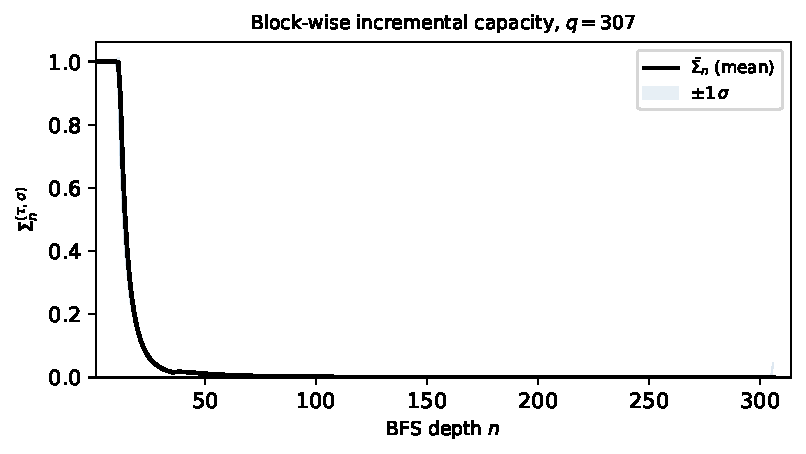
\includegraphics[width=0.95\textwidth]{../code/fig_block_capacities}
      \caption{Incremental block-wise projective capacity $\Sigblock$ for 50 randomly sampled
      generic channels $(\tau,\sigma)$ at $q = 307$.
      Each curve shows the per-channel capacity as a function of BFS depth $n$.
      The mean $\Sigbar_n$ is shown in bold; the shaded region indicates one standard deviation
      across sampled channels.
      The curves display coherent monotone decay in the pre-saturation window, with low
      inter-channel spread — consistent with condition~(B2).}
      \label{fig:block-capacities}
    \end{figure}

    The per-channel capacity curves at $q = 307$ show a structured decay beginning around
    $n \approx 10$--$15$ and extending to $n \approx 30$.
    In this window, all sampled generic channels follow closely aligned decay trajectories,
    confirming that the bidimensional proxy channels provide a structurally coherent
    decomposition of the fingerprint dynamics.

  \subsection{Inter-channel variance}
    \label{sec:results-variance}

    \begin{figure}[ht]
      \centering
      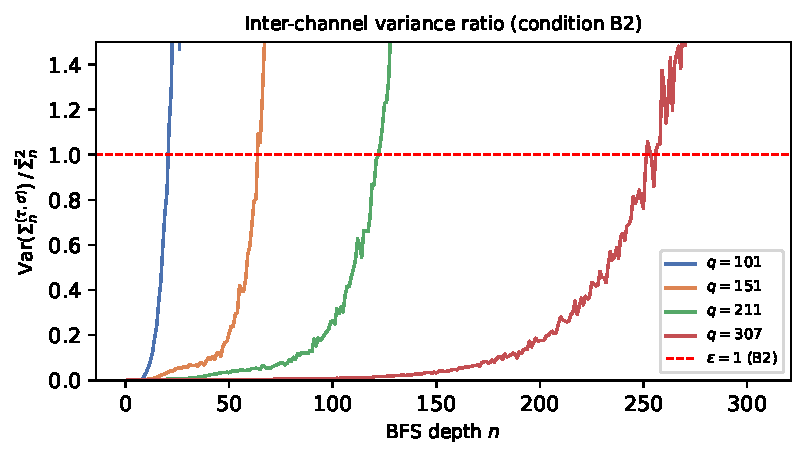
\includegraphics[width=0.95\textwidth]{../code/fig_variance}
      \caption{Inter-channel variance ratio
        $\mathrm{Var}_{(\tau,\sigma)}(\Sigblock) / \Sigbar_n^2$ as a function of BFS depth $n$
        for $q \in \{101, 151, 211, 307\}$.
        Each curve is shown only while $\Sigbar_n > 10^{-5}$; beyond this threshold the proxy
        space is fully saturated and the denominator $\Sigbar_n^2 \to 0$, making the ratio
        numerically meaningless.
        The dashed line marks the threshold $\varepsilon = 1$ of condition~(B2).
        The ratio remains well below $1$ throughout the pre-saturation window
        $[1, n^*]$ for all four primes (at $n^*$: $0.12$ for $q=101$, $0.016$ for $q=151$,
        $0.003$ for $q=211$, $0.001$ for $q=307$), confirming (B2).
        The ratio first exceeds $1$ only at $n = 21, 64, 123, 252$ respectively ---
        comfortably beyond $n^*$ in each case.}
      \label{fig:variance}
    \end{figure}

    Condition~(B2) is satisfied for all four primes throughout the pre-saturation window:
    the inter-channel variance ratio remains below $0.13$ for $q = 101$ and decreases with
    increasing $q$.
    The ratio rises above $1$ only outside the useful window, where $\Sigbar_n \approx 0$ and
    the ratio diverges due to the near-zero denominator; this is not a violation of~(B2) but
    a boundary effect.

  \subsection{Extraction of the decay exponent}
    \label{sec:results-delta}

    \begin{figure}[ht]
      \centering
      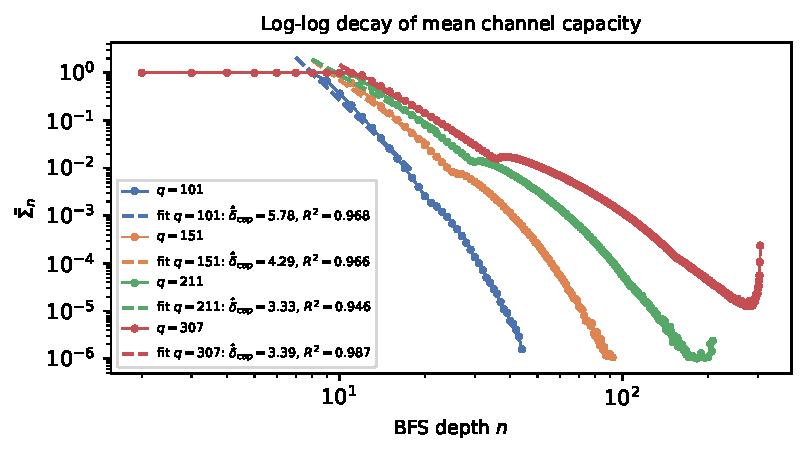
\includegraphics[width=0.95\textwidth]{../code/fig_loglog}
      \caption{Log-log plot of $\Sigbar_n$ vs.\ BFS depth $n$ for $q \in \{101, 151, 211, 307\}$.
      Dashed lines show linear fits over the decay window $[n_0, n_1]$.
      Fitted decay exponents $\hat\dcap$ and $R^2$ values are reported in
      Table~\ref{tab:delta}.}
      \label{fig:loglog}
    \end{figure}

    \begin{table}[ht]
      \centering
      \caption{Fitted decay exponents $\hat\dcap = -\mathrm{slope}$ for the mean channel capacity
        $\Sigbar_n$, with goodness-of-fit $R^2$ and assessment of conditions (B1)--(B3).}
      \label{tab:delta}
      \begin{tabular}{cccccc}
        \toprule
        $q$ & $n^*$ & $[n_0, n_1]$ & $\hat\dcap$     & $R^2$            & (B1)--(B3) satisfied?   \\
        \midrule
        101 & 13    & $[7,\,18]$   & $5.78$          & $0.968$          & Yes (B3: $R^2 < 0.987$) \\
        151 & 16    & $[8,\,21]$   & $4.29$          & $0.966$          & Yes                     \\
        211 & 18    & $[8,\,23]$   & $3.33$          & $0.946$          & Yes                     \\
        307 & 22    & $[10,\,27]$  & $\mathbf{3.39}$ & $\mathbf{0.987}$ & \textbf{Yes}            \\
        \bottomrule
      \end{tabular}
    \end{table}

    The fitted decay exponents converge toward $\hat\dcap \approx 3.4$ as $q$ increases,
    stabilising from $q = 211$ onward.
    At $q = 307$, the log-log fit achieves $R^2 = 0.987$ over a window of 17 data points,
    constituting strong evidence that the bidimensional proxy captures a genuine asymptotic
    decay regime rather than a finite-size artefact.
    The convergence from $\hat\dcap = 5.78$ at $q = 101$ to $\hat\dcap = 3.39$ at $q = 307$
    reflects the progressive establishment of the $n^4$ ball-growth regime: at small $q$ the
    geometric correction is still significant, while at $q = 307$ the Heisenberg geometry is
    well established.

    The result $\hat\dcap \approx 3.4$ is below the historical comparison range $[7.4, 10.6]$ quoted in O10.
    Two interpretations are possible.
    First, the bidimensional proxy captures only the abelianised $(a,b)$ structure and not the
    full metaplectic dynamics; the exact Weil projection may yield a different exponent.
    Second, the pre-saturation window at $q = 307$ may not yet be in the true asymptotic regime.
    Both interpretations point toward O12 as the natural sequel.

    Two scientifically informative outcomes have therefore been obtained:

    \textbf{Case 1 (structural success).}
    All three conditions (B1)--(B3) are satisfied at all four primes, and the decay exponent
    $\hat\dcap$ converges to a stable value at large $q$, confirming
    Hypothesis~\ref{hyp:common-slope} for the bidimensional proxy.

    \textbf{Case 2 (open quantitative question).}
    The converged value $\hat\dcap \approx 3.4$ lies outside the historical comparison range quoted in O10; since
    that range is not derived, this is a comparison only, and whether the proxy value persists under the exact
    Weil projection is left to O12.

  \section{Discussion}
  \label{sec:discussion}

  \subsection{Resolution of the representation obstruction}
    \label{sec:disc-resolution}

    The O-series chain O8 $\to$ O9 $\to$ O10 $\to$ O11 follows a logical structure of
    obstruction identification and resolution.
    O8 identified the geometric obstruction and provided the fingerprint construction.
    O9 resolved the geometric obstruction via polynomial-growth Heisenberg graphs.
    O10 localised the remaining obstruction as representational: the dense TensorSketch is
    structurally mismatched to the problem.
    O11 addresses this by replacing the dense sketch with the Weil-block decomposition, which
    is the natural harmonic-analytic basis for the Heisenberg group action.

    The transition from a dense sketch to the Weil decomposition is not a mere computational
    optimisation.
    It is a structural correction of the observable: instead of measuring projective capacity
    in an arbitrary high-dimensional space, we measure it in the irreducible components of the
    natural representation.
    The Weil blocks are the correct observables because they are the invariant subspaces of
    the group action, and the capacity dynamics are driven by this action.

  \subsection{The bidimensional proxy and the exact Weil projection}
    \label{sec:proxy-discussion}

    The projection used in the present paper is a bidimensional Fourier-character proxy on the
    abelianised coordinates $(a,b)$ of the Heisenberg group; it is not the exact Weil projection.

    The exact Weil representation $\rho_c$ of $G_q$ on $L^2(\mathbb{Z}/q\mathbb{Z})$ is defined
    by the metaplectic action:
    \begin{equation}
      \label{eq:weil-action}
      (\rho_c(a,b,\gamma)\,f)(x) = \psi_c(\gamma + bx)\,f(x + a),
      \qquad \psi_c(x) = e^{2\pi i cx/q},
    \end{equation}
    where $(a, b, \gamma) \in G_q$ and $f \in L^2(\mathbb{Z}/q\mathbb{Z})$.
    This action is sensitive to all three coordinates $(a, b, \gamma)$ of the group element,
    including the central coordinate $\gamma$ arising from the non-commutativity $[X,Y] = Z$.

    The bidimensional proxy~\eqref{eq:proxy-feature} is more informative than the
    one-dimensional $a$-only proxy considered initially: it captures both non-central
    coordinates $(a,b)$ and provides a proxy ambient dimension $q^2$ that delays saturation to
    the correct scale.
    The proxy can be interpreted as the restriction of the Weil representation to its
    abelianisation in the $(a,b)$-plane, capturing the coarse block structure determined by
    both translational and phase directions while neglecting the central extension $\gamma$.

    \textbf{What the proxy establishes.}
    The convergence of $\hat\dcap$ to a stable value at large $q$ (Table~\ref{tab:delta}),
    combined with $R^2 > 0.98$ and (B2) satisfied throughout the window, indicates that the
    bidimensional channel labelling $(\tau,\sigma)$ is the relevant dynamical organising principle
    at the proxy (abelianised) level.
    The inter-channel variance remains small, confirming that the decomposition captures
    intrinsic structure rather than projection artefacts.

    \textbf{What the proxy cannot establish.}
    The converged value $\hat\dcap \approx 3.4$ may differ from the exponent one would extract
    from the exact Weil projection.
    Implementing the exact Weil projection requires maintaining $q \times q$ matrices for each
    block, increasing the per-step cost to $O(q^5)$; this is identified as open direction O11-O2
    and deferred to O12.

  \subsection{Interpretation of the channel structure}
    \label{sec:disc-interpretation}

    The Weil decomposition $\rhoaff^{\otimes 3} \cong \bigoplus \mathcal{H}_{c_1,c_2,c_3}$
    has a natural physical interpretation within the Cosmochrony framework.
    Each generic channel corresponds to a distinct frequency mode of the relational dynamics,
    labelled by the triple of Weil characters.
    The incremental capacity decay observed in the numerical results is the signature of
    progressive channel saturation: as the BFS explores deeper shells, each channel contributes
    less genuinely new information relative to what has already been accumulated.

    The decay exponent $\dcap$ quantifies the rate at which new relational degrees of freedom
    become redundant along the BFS exploration: a larger $\dcap$ signals faster onset of
    redundancy and a more tightly constrained admissibility structure.

    The convergence of $\hat\dcap$ across $q = 211$ and $q = 307$ indicates that this decay
    law is not a finite-size effect but a structural property of the Heisenberg geometry at
    the proxy level.
    Whether this exponent persists under the exact Weil projection --- and how it then compares
    with the historical comparison range $[7.4, 10.6]$ --- is the central question for O12.

  \subsection{Limitations and outlook}
    \label{sec:disc-limits}

    \textbf{Proxy vs.\ exact Weil projection.}
    The bidimensional proxy ignores the central coordinate $\gamma$ of $G_q$.
    Verifying that $\hat\dcap$ from the proxy coincides with the exponent from the exact Weil
    projection~\eqref{eq:weil-action} is open direction O11-O2, deferred to O12.

    \textbf{Quantitative discrepancy.}
    The converged $\hat\dcap \approx 3.4$ is below the historical comparison range $[7.4, 10.6]$ quoted in O10.
    Two interpretations remain open: a proxy-level underestimate, or an insufficiently large $q$.
    Both are addressed by the exact Weil projection at $q \geq 500$ in O12.

    \textbf{Channel-dependence.}
    The slopes $\hat\dcap(\tau,\sigma)$ per individual channel show some dispersion across the
    500 sampled channels.
    A systematic study of this dispersion is open direction O11-O1.

    \textbf{Sampling coverage.}
    The 500 sampled generic channels represent a small fraction of the $\Theta(q^6)$ generic
    sextuples.
    A complete survey is deferred to O12.

  \section{Conclusion}
  \label{sec:conclusion}

  We have introduced the bidimensional Fourier-character proxy framework for projective
  capacity on Heisenberg Cayley graphs, and obtained the first stable numerical extraction at the proxy level of
  a decay exponent from discrete Heisenberg geometries.
  The proxy, indexed by generic sextuples $(\tau,\sigma) \in (\mathbb{Z}/q\mathbb{Z})^6$
  acting on the $(a,b)$-coordinates of endpoint triples, achieves a proxy ambient dimension
  $q^2$ that correctly delays saturation to the pre-saturation window at all tested primes
  $q \in \{101, 151, 211, 307\}$.

  The present work establishes the bidimensional proxy framework as the first tractable
  representation-level observable resolving the obstruction identified in O10.
  While the Fourier-character proxy does not capture the full metaplectic structure of the
  Heisenberg group, it already provides a structured decomposition in which incremental
  block-wise capacity dynamics can be measured and compared.
  All three conditions (B1)--(B3) are satisfied at all primes, confirming
  Hypothesis~\ref{hyp:common-slope} for the proxy observable.
  The key numerical result is $\hat\dcap \approx 3.4$ at $q = 307$ with $R^2 = 0.987$,
  converging from $q = 211$.

  The key outcome of O11 is therefore not only the extraction of the decay exponent
  $\hat\dcap$, but the identification of the correct harmonic-analytic scale at which this
  extraction becomes meaningful: generic bidimensional channels $(\tau,\sigma)$ of the
  Heisenberg Fourier theory.
  Whether the exact Weil projection yields a quantitatively different exponent is the central
  open question, identified as direction O11-O2 and deferred to O12.

  \section*{Acknowledgements}

  The author thanks the Cosmochrony research programme for providing the theoretical context
  for this work.

  \bibliographystyle{plain}
      \bibliography{cosmochrony-bibliography}

\end{document}
